\section{Design}
Snake-spillet er lavet efter et Model-View-Control-design (MVC). Styringen, spil logikken og den visuelle repræsentation holdes adskilt i tre dele. Med dette bygges et meget modulært program. Spil logikken er Model, styringen er Control og den visuelle repræsentation er View. Disse tre dele skal kode mæssigt holdes adskilt. Spil logikken må ikke kende til styringen eller repræsentationen. Repræsentation må ikke kende til styringen. Styringen må godt kende til spil logikken og repræsentationen, se \figref{mvc} for en illustration.

\begin{figure}[h]
	\centering
   	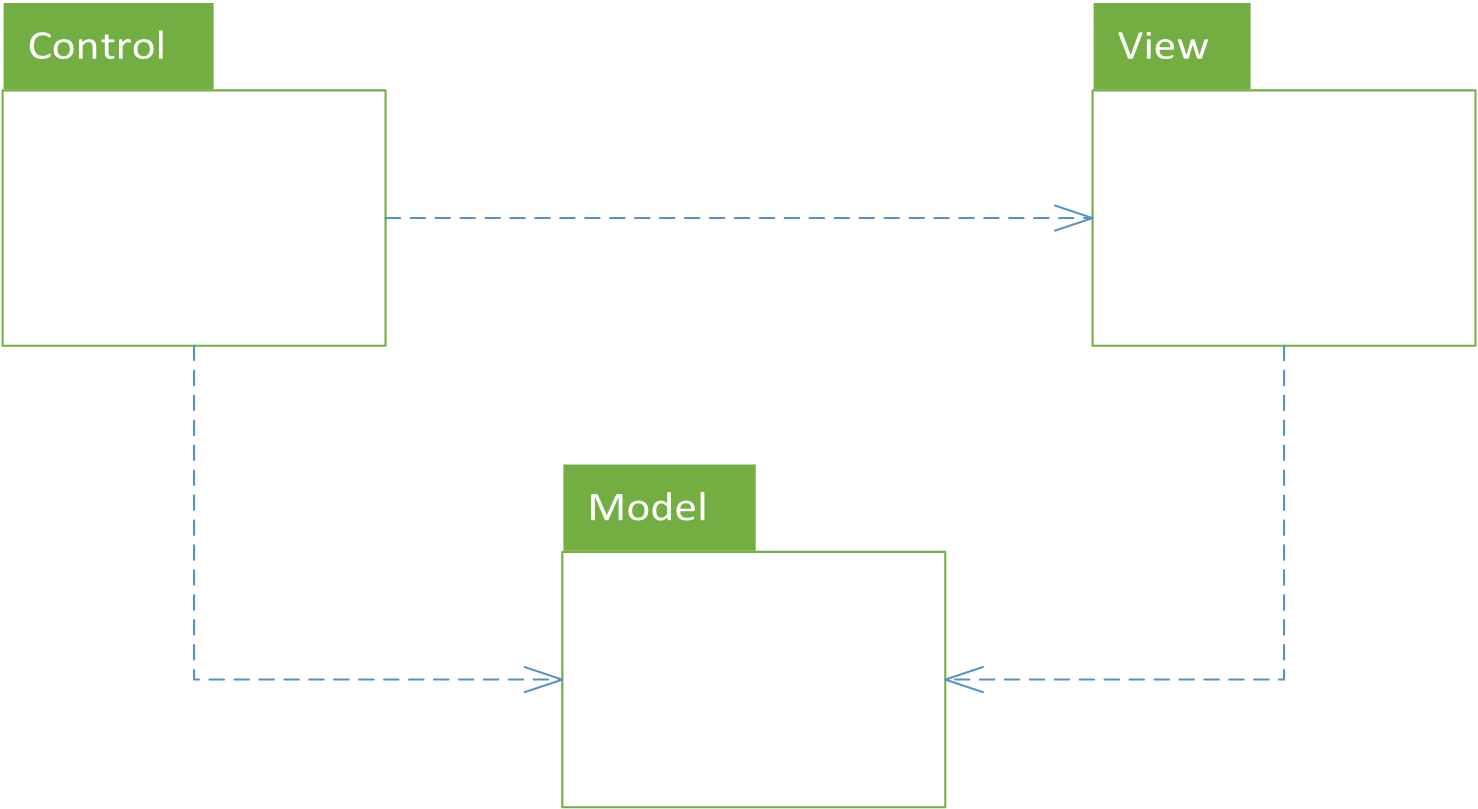
\includegraphics[width=0.7\textwidth]{grundlaeggende/mvc.png}
	\hspace{0.1\textwidth}
	\caption{\figlab{mvc}Oversigt over Model-View-Control design.}
\end{figure}

Brugeren interagere med den del der er dedikeret til styring (Control). Control manipulerer spil logikken (Model) og spillet visualiseres i View-koden. Model sikre at brugeren ikke snyder. Alle funktioner, der påvirker programmets tilstand, skal holdes i Model-koden. Control modtager input fra brugeren og sender det videre til View og Model. View må ikke ændre på spillets tilstand, det skal kun vise hvad der er i Model. 

Man kan tænke på det sådan at View observere Model og viser hvad den ser til brugeren. Control kommunikere med brugeren og sender relevant kommunikation videre til View eller Model.

Simpel Snake er designet, så spillets logik ligger i \textit{Game} klassen i Model-pakken. \textit{Game} indeholder relevante hjælpe klasser, som for eksempel Level (banen) og Snake (slangen). Se \figref{TODO}. Vi har valgt at lave to enum-klasser, \textit{Direction} og \textit{Action}. De holder styr på tilstande i spil logikken og forsimpler kommunikation til \textit{Game} klassen. Det er nemmere at tilkoble kommandoer og statements til hver retning, hvis der eksplicit er en Direction klasse som begrænser retnings mulighederne. At have en Action-state frem for en integer giver næsten selvdokumenterende kode. Vi har valgt at gøre \textit{Game} til en \textit{Observable}. Med dette kan vores View klasser observere spil logikken og opdatere, det som brugeren ser, lige så snart spillets tilstand ændrer sig.

I \textit{View}-klassen har vi vores vindue som brugeren ser spillet igennem. Det har en \textit{BoardPanel}-klassen som viser den nuværende spil tilstand. \textit{BoardPanel} nedarver fra \textit{Observer} og opdatere panelet hver gang spillets tilstand ændres. Når dette sker tegnes den nuværende bane, slange og mad som er i \textit{Game} objektet. For eksempel bruges \textit{getSnake()}, til at bestemme hvor slangens position. Scoren holdes opdateret i en \textit{Score}-klasse i \textit{Game} objektet. \textit{ScorePanel} ligger som et panel øverst over \textit{BoardPanel} i vinduet. Den observere \textit{Score} klassen i \textit{Game} og opdatere sig selv når score ændre sig. Se \figref{TODO}.

Spillets tilstand ændres, når der modtages input i Control-klasserne. De bestemmer hvornår og hvordan slangen bevæger sig. \textit{Control}-klassen nedarver fra en KeyListener. Gennem piletasterne, kommunikere den til \textit{Game} at brugeren gerne vil flytte slangen. Se \figref{TODO}.

For at starte spillet bruges klassen \textit{Driver}, som opretter et \textit{Game}-, \textit{View} og \textit{Control}-objekt.